\documentclass{article}
\usepackage{graphicx}
\usepackage[utf8]{inputenc}
\usepackage[T1]{fontenc}
\usepackage[francais]{babel}
\usepackage{layout}


\begin{document}
\begin{titlepage}
\begin{center}
\Huge Principes généraux du programme

\normalsize
\vspace{0.5cm}
\Large {\underline{ Groupe 3 Bleu : Sokoban} }

\vspace{1cm}
\normalsize
Goron Nathan, De La Rosa Louis-David, Basset Emilien, Demé Quentin

\vspace{14.5cm}
L2 informatique 2016-2017 Université de Caen Basse-Normandie
\end{center}
\end{titlepage}


\newpage
\section{Introduction}
Pour commencer, nous avons choisit de programmer notre sokoban en orienté objet car cela présente quelques avantages majeurs comme la
possibilité de stocker plein d'information assez explicitement dans des listes. On a également choisit l'orienté objet car c'est ce qui 
nous semblait être le plus intuitif.

\section{\underline{Conception du jeu}}
	\subsection{Les classes}
	Il y a en tout 5 classes :
		\begin{itemize}
		 \item Sprite
		 \item Personnage (qui hérite de Sprite)
		 \item Caisse (qui hérite également de Sprite)
		 \item Niveau
		 \item LevelCollection
		\end{itemize}
	Les classes Sprite, Personnage et Caisse vont servir à représenter tout les objets du jeu voici la liste de tout les objets Existants :
		\begin{itemize}
		 \item le personnage - il representera comme son nom l'indique le personnage controlé par le joueur.
		 \item les caisses - elle seront poussé par le personnage
		 \item les murs - il sont là pour bloquer tout ce qui se déplace, c'est à dire le personnage et les caisses
		 \item les cibles - ce sont les emplacement sur lesquels il faut placer les caisses
		 \item le vide et les espaces - il representent les endroits ou il n'y a rien
		\end{itemize}
	Les murs, les espaces, le vide, et les cibles sont des instances de la classe Sprite. les caisses des instances de la classe Caisse et le personnage 
	sera une unique instance de la classe Personnage.
	\newline
	La classe Niveau representera le niveau qui sera acutellement chargé. il contient entre autre la méthode qui affiche puis raffraichit tout le jeu.
	Il contient également quelques fonctions utiles comme la recherche de la position du personnage ou encore une partie du test de victoire.
	\newline
	La classe LevelCollection sert à charger une collection de niveau presente dans un fichier .slc. On demade un niveau via la methode load().
	\subsection{représentation du plan}
	Pour représenter le sokoban, nous avons choisit de le construire de la sorte : le programme se compose de 2 grilles nommé gameP 
	et gameO. Ces dernières contiennent des objets cités plus haut.
	\newline
	la grille gameP (game Plan) contient les cibles et les espaces. la grille gameO (game Obstacle) contient les murs, les caisses et le personnage.
	\newline
	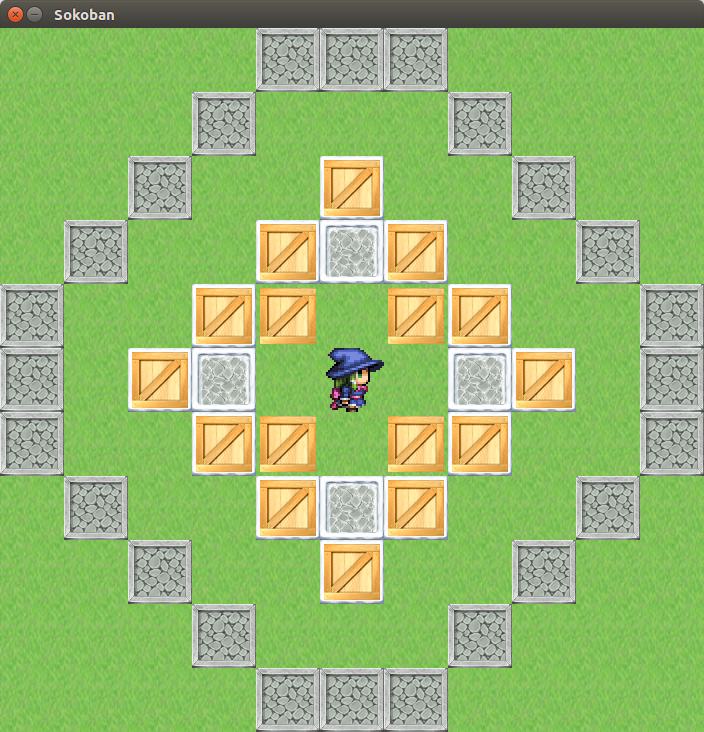
\includegraphics[scale=0.25]{05.png}
	\newline
	aperçue graphique du plan.
	\newline
	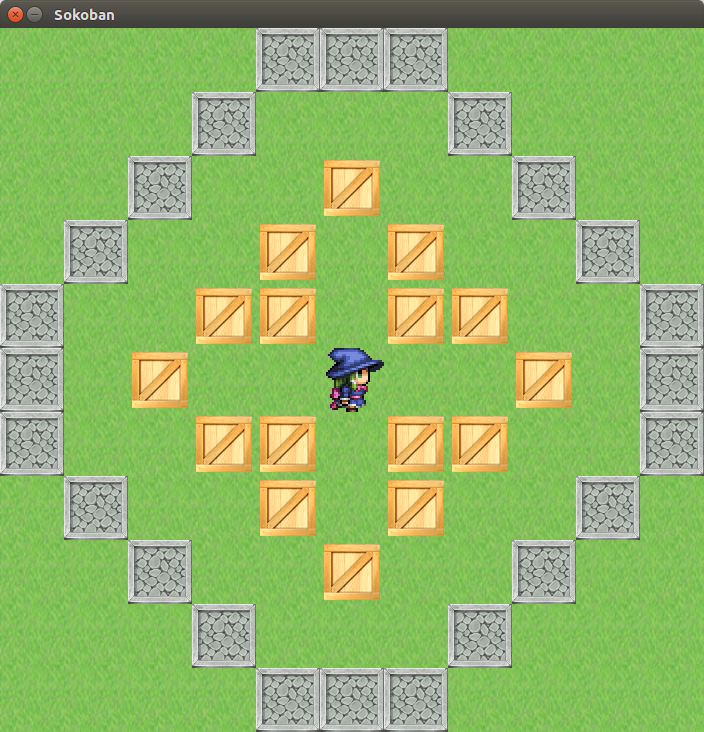
\includegraphics[scale=0.25]{06.png}
	\newline
	aperçue graphique de la grille gameO.
	\newline
	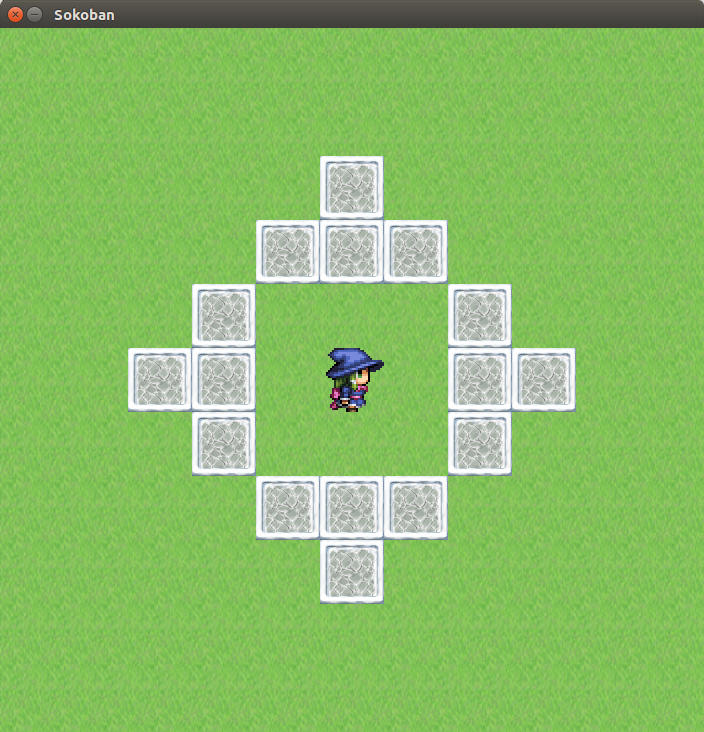
\includegraphics[scale=0.25]{07.png}
	\newline
	aperçue graphique de la grille gameP (ne pas considérer le joueur).
\vspace{1cm}
\section{\underline{Le joueur}}
	\subsection{gestion des déplacements}
	Le joueur est une instance de la Classe Personnage. il a donc une methode specialisé nommé deplace(). ci dessous l'explication de sont fonctionnement :
	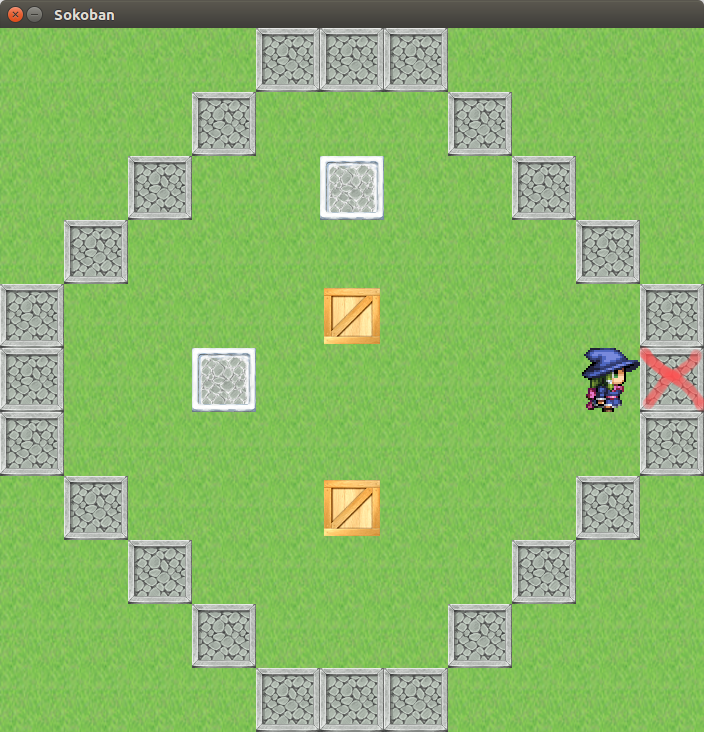
\includegraphics[scale=0.25]{01.png}
	\newline
	Le personnage test sa destination et ne se déplace pas si la case est prise.
	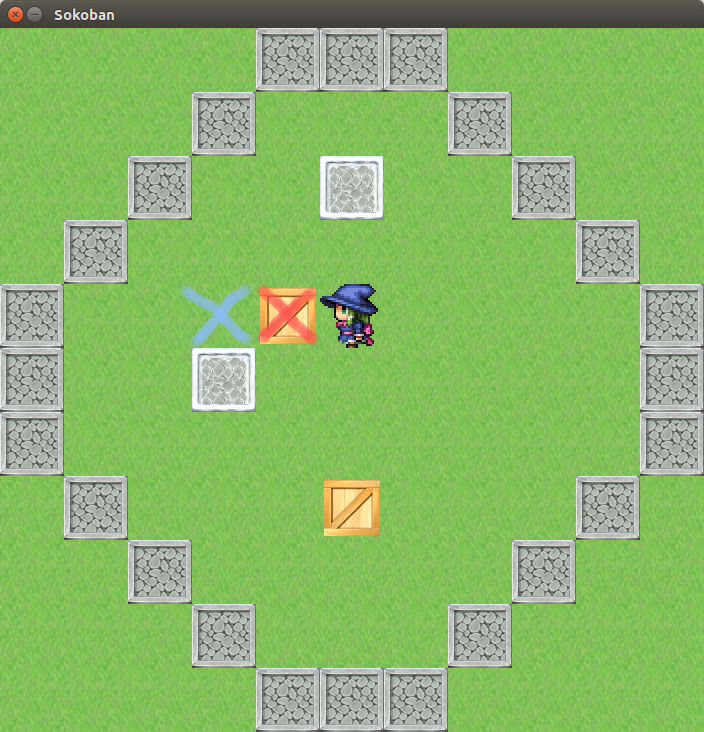
\includegraphics[scale=0.25]{02.png}
	\newline
	Le personnage test sa destinaton est rencontre une caisse (croix rouge). il demande donc à la caisse de tester si sa destination est libre 
	(croix bleue).
	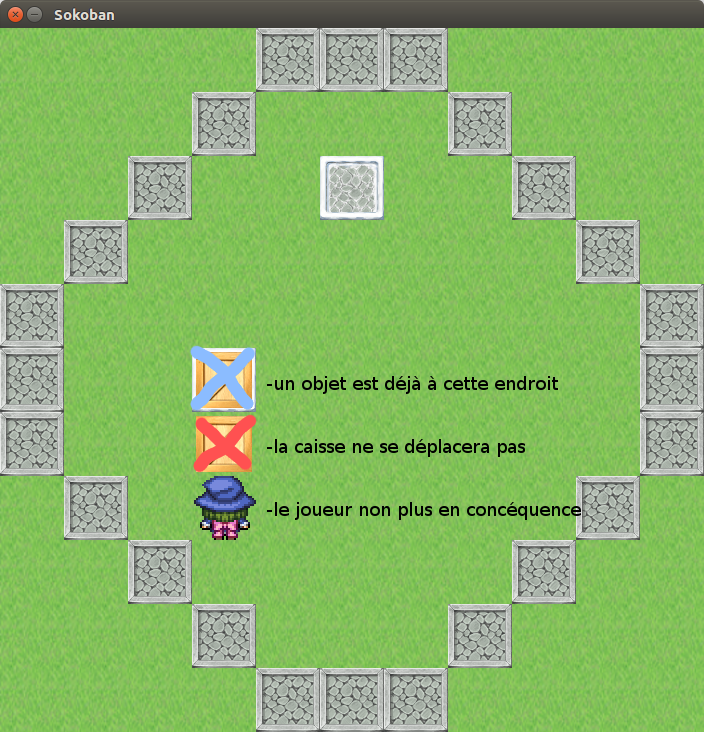
\includegraphics[scale=0.25]{04.png}
	\newline
	Exemple de déplacement impossible.
	\subsection{représentation graphique}
	Le personnage a une représentation graphique un peu particulière. Etant donné qu'il doit se déplacer dans 4 directions, il faut que celui ci ait une image 
	différente pour chaques déplacements. On a aussi fait le choix d'animer le personnage lorsqu'il se déplace, il font donc une frame par pas. Dans notre cas 
	le personnage a 3 frames par pas dont une qui se repète. on a donc 4 fois 3 images pour notre personnage.
	\newline
	Sur internet on a reussi à trouver ce type d'image appelé ``tileset'' et en bonus un 8 styles différents pour le personnage :
	\newline
	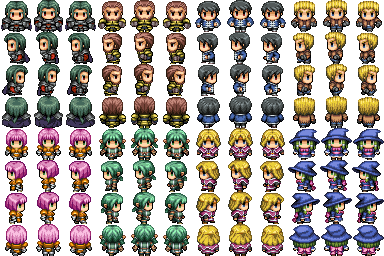
\includegraphics[scale=0.25]{08.png}
\vspace{1cm}
\section{\underline{Les règles du jeu}}
	\subsection{Les déplacements}
	Avec le système d'objet que l'on a choisit, les déplacements respectent les règles du jeu qui sont :
	\begin{itemize}
	 \item On ne peut que pousser les caisses
	 \item On ne peut pas pousser plus d'une caisse à la fois
	 \item Les caisses et le personnage ne peuvent pas traverser les murs
	 \item La partie est gagné lorsque toutes les caisses se trouvent sur les cibles
	 \item Le joueur a la possibilité de revenir en arrière si un déplacement n'aurait pas du être.
	 \item l'objectif est de reussir à mettre toutes les caisses sur les cibles en faisant le moins de déplacements possible.
	\end{itemize}

	\subsection{Condition de victoire}
	le fonctionnement de la condition de victoire est simple : une fonction va voyager dans la grille gameP. si il y a une cible, alors verifer dans 
	la grille GameO si une caisse est dessus, si c'est le cas, c'est gagné.
	\newline
	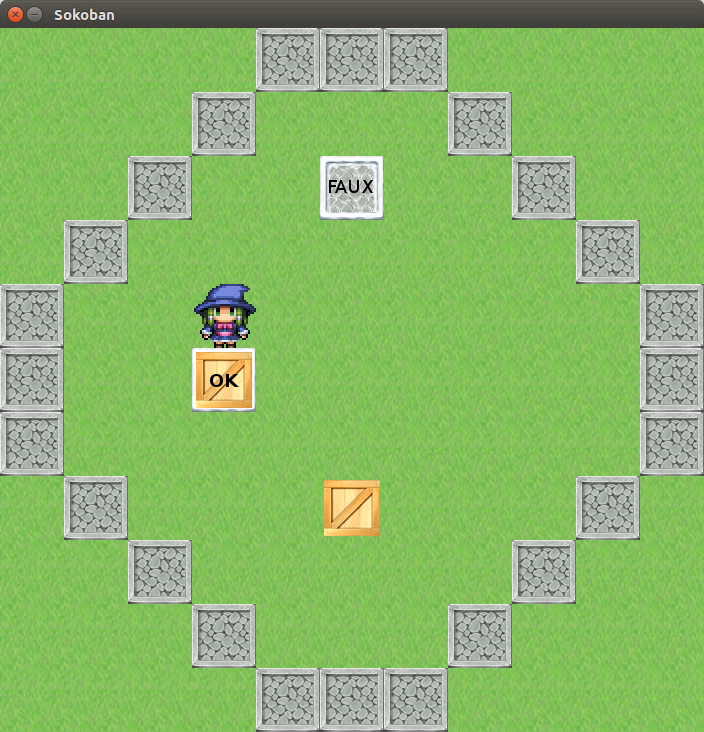
\includegraphics[scale=0.25]{03.png}
	\newline
	La condition n'est pas verifiée.

	
		

\newpage
\end{document}